\section{Uvod}
Velikosti populacije je v ekologiji pomemben parameter, ki ga lahko preučujemo. Služi v pomoč pri raziskovanju drugih značilnosti populacije. Z nekaterimi populacijami živali aktivno upravljamo in ocena številčnosti je lahko izhodiščni parameter za kvaliteten trajnostni odvzem osebkov iz populacije.

\subsection{Pomen ocene velikosti populacije kot biološki parameter}
Populacijo lahko opredelimo kot skupino osebkov iste vrst, ki naseljujejo skupni prostor v danem času \citep{krebs_ecology:_2001}. Kot taka je na voljo za proučevanje in upravljanje.

Proučevanje katero koli populacije se začne s poznavanjem njene biologije in ekologije. Posamično ali v skupinah proučujemo demografske parametre, ki dajo vpogled v populacijo in vrsto. Taki parametri so denimo življenjska doba, število potomcev, stopnja preživetja različnih starostnih skupin ipd. Poleg teh pa je pomembna tudi velikosti populacije, ki jo lahko imenujemo tudi številčnost oz. jo gledamo na znano velikem prostoru kot gostoto. Številčnost je eden najbolj intuitivnih parametrov, ki jih lahko pripišemo populaciji, saj predstavlja izhodišče za upravljanje. Poleg številčnosti so lahko drugi omejujoči dejavniki, denimo genetska slika. Primera takih dveh (sub) populacij lahko spremljamo na primerih floridskega panterja \citep{pimm_genetic_2006} ali nenazadnje slovenskega risa.

\subsection{Načini ocenjevanja številčnosti}
Velikost populacije lahko ocenjujemo na dva načina. Kot število osebkov na območju vzorčenja ali neposredno kot gostoto (število osebkov na prostorsko enoto). V obeh primerih pa ostaja problem zaznavnosti posameznega osebka. Zaradi načina življenja ali pa velikega območja na katerem se populacija razteza, vseh živali fizično ni mogoče zaznati v izvedljivih časovnih, finančnih in drugih okvirih. Zato moramo poseči po pristopih, ki omogočajo, da zaznanim osebkom "prištejemo" tiste, ki smo jih spregledali. Na ta način lahko ocenimo vsoto zaznanega in pričakovanega dela populacije. S pomočjo znanstveno preverljivih metod lahko oceni podamo tudi interval zaupanja, s katerim lahko sporočimo tudi kako natančna je naša ocena.

Ko na določenem območju z gotovostjo zaznamo vse osebke, jih preprosto preštejemo. To imenujemo cenzus, kjer predpostavimo, da vse osebke zagotovo zaznamo ($p=1$). Cenzusi v ekologiji niso pogosti, ker določen delež osebkov navadni ni mogoče zaznati. Metode, ki upoštevajo dejstvo, da vsi osebki med vzorčenjem niso zaznani s popolno gotovostjo ($p < 1$), so osnovane na podlagi štetja na ploskvah, oddaljenosti od opazovalca in lova in ponovnega ulova \citep{williams_analysis_2002}.

Metoda štetja na ploskvah deluje na način, da območje, kjer želimo oceniti številčnost neke populacije, razdelimo na prostorske podenote. Na vzorcu podenot izvedemo vzorčenje in iz ocen številčnosti v podenotah lahko sklepamo o številčnosti na večjem območju. Pri tem moramo upoštevati več predpostavk, saj ima sklepanje iz vzorca na večje območje več pasti.

Metode, kjer se beleži oddaljenost osebka od točke opazovanja, v prvi vrsti podajo oceno gostote. Opazovanje lahko poteka na naključno izbranih točkah ali transektih, vhodni podatki za računanje pa je razdalja osebka do transekta. Predpostavlja se, da je na transektih, ki jih popisovalec pregleduje, zaznavnost 1, z oddaljenosti od transekta pa zaznavnost pada po krivulji. Tip krivulje lahko izberemo na podlagi teorije ali prakse.

Do sedaj opisani načini za oceno številčnosti niso upoštevali identitete zaznanega osebka, kar pa je domena metod ulova in ponovnega ulova.

\subsection{Metoda lova in ponovnega ulova}
\subsubsection{Osnovne značilnosti metode lova in ponovnega ulova}

Metode ulova in ponovnega ulova se od zgoraj naštetih metod razlikujejo po tem, da za informacijo uporabljajo identiteto osebka. Zanesljiva določitev identitete osebka je najvišja kvaliteta podatka, ki ga lahko pridobimo za oceno številčnosti populacije. Kljub temu, da so bile nekatere matematične osnove metode lova in ponovnega ulova razvite že pred več stoletji, se je paleta modelov razširila in prešla v splošno uporabo v začetku dvajsetega stoletja \citep{pollock_capture-recapture_2000}.

Poznamo več matematičnih modelov in vsak ima svoje značilnosti. V eni od delitev lahko modele razvrstimo na dve večji skupini, ki se razlikujeta po tem, da so primerne za odprte oz. zaprte populacije. O odprtih populacijah govorimo takrat, ko osebki med vzorčenjem prihajajo in odhajajo iz populacije. Zaprte populacije tega prehoda ne predpostavljajo in je zato že v osnovi pojem "velikost populacije" lažje opredeliti. Pregled metod za zaprte populacije v svojem klasičnem delu opišejo \citet{otis_statistical_1978}, kasneje pa še drugi (tudi za odprte), kot so \citet{white_capture-recapture_1982}, \citet{seber_review_1986} in \citet{white_program_1999}.

\subsubsection{Prepoznavanje osebkov}
Da lahko osebek prepoznamo kot edinstvenega, ga moramo na nekakšen način ujeti oz. zaznati. V preteklosti je to predstavljalo fizičen ulov, nakar so žival nedvoumno označili. Osebke se označuje na načine, da je oznaka trajna ali začasna (npr. označevanja robnih lusk ščita pri želvah \citep{pike2005}, ščipanje ušes ali nohtov pri manjših sesalcih \citep{wiewel_assessing_2007}, pisanje številk na krila metuljev \citep{jugovic_movement_2017}, ščipanje prstov pri dvoživkah \citep{campbell_evaluation_2009}, opremljanje z ušesnimi značkami, barvanje kožuha, tetoviranje idr.).

Z napredovanjem molekularnih tehnik in večanjem računalniške moči, je danes možen ulov brez fizičnega stika z osebki. Tako je manj verjetno verjetno, da bo spremenila vedenje in posledično spremenila njeno ulovljivost.
Iz neinvazivno nabranih vzorcev (npr. sluzi, sline, dlake, iztrebka, perja) preko DNK z relativno visoko zanesljivostjo določimo identiteto osebka. Pri živalih, ki imajo značilno obarvano kožo ali dlako (npr. trebuh nekaterih dvoživk, obarvanost kožuha pri risu), lahko s pomočjo fotografij in računalniških programov ločimo med različnimi osebki.

\subsubsection{Območje vzorčenja}
Ulov in označevanje osebkov poteka na geografsko določenem območju, ki za živali z velikim območjem gibanja le deloma zaobjame proučevano populacijo. Velikost območja vzorčenja je navadno omejeno zaradi velikih razdalj potovanj, fizičnimi mejami (otoki) ali pa s političnimi mejami (parkov, držav ali drugih enot). Iz tega sledi, da osebke zaznavamo (lovimo), njihovo gibanje ni nujno omejeno na naše arbitrarno določeno območje vzorčenja.

\subsubsubsection{Domač okoliš}
Območje domačega okoliša osebka predstavlja prostor, kjer se zadržuje osebek med dnevnimi aktivnostmi. Raba prostora navadno sovpada s trenutnimi potrebami osebkov (iskanje hrane, partnerjev) in se v času lahko spreminja. Velikost območja je odvisna od velikosti organizma ter razpoložljivosti hrane in drugih virov potrebnih za življenje.

\subsubsubsection{Superpopulacija}
Populacija je skupina osebkov, ki se nahajajo znotraj območja vzorčenja. Poleg osebkov, ki se neprestano zadržujejo znotraj območja vzorčenja, lahko zaznamo tudi osebke, ki prehajajo njegove meje, ker se njihov domač okoliš le deloma prekriva z našim arbitrarnim območjem vzorčenja. Njihova zaznavnost je v povprečju nižja od osebkov, ki se v prostoru in času stalno nahajajo v območju vzorčenja. Skupaj z ostalimi osebki tvorijo t.i. superpopulacijo, za katero pa ne vemo natančno kako je prostorsko omejena.


\subsubsection{Predpostavke metod ulova in ponovnega ulova}
Kot velja za vse modele, tudi pri modelih ulova in ponovnega ulova veljajo predpostavke. Kršitev le-teh ima lahko za posledico blage ali hude posledice. V splošnem se trudimo, da predpostavkam zadostimo. V primerih simuliranih vrednosti lahko nekatere predpostavke zanemarimo ali pa jih celo nadzorujemo, kar nam pomaga proučevati kaj se dogaja pri kršenju le-teh.

\subsubsection{Zanesljivost označevanja}
Da osebek nedvoumno in zanesljivo označimo pomeni, da se oznaka v prostoru in času ne izgubi ali spremeni in da jo raziskovalec lahko zanesljivo prebere. V preteklosti se je uporabljalo neposredne načine označevanja (ušesne oznake, tetovaže, rezanje uhljev, barvanje krempljev…) danes pa se za vsaj nekatere skupine živali (npr. večji sesalci) uporabi pristope s pomočjo genetike. Ker za nabiranje nekaterih tipov vzorcev (iztrebkov, dlak, peres) ne potrebujemo neposrednega stika z osebkom, to imenujemo neinvazivno vzorčenje. Pri genetskem vzorcu je zaradi napak genotipizacije ali identičnih dvojčkov mogoče, da genotip določimo narobe, vendar so metode kljub temu relativno zanesljive v smislu označevanja osebkov \citep{waits_noninvasive_2005}. Za živali, ki imajo značilne vzorce kožuha se uporablja lahko foto pasti, ki so doživele razmah uporabe v zadnjih desetih letih.

\subsubsection{Enaka ulovljivost}
Predpostavlja se, da imajo vse živali enako verjetnost, da jih bomo zaznali oz. ulovili. Do neenake ulovljivosti lahko pride na več načinov. Če imajo živali različne ulovljivosti govorimo o heterogenosti ulovljivosti. Zvišanje (t.i. trap-happy) ali znižanje ulovljivosti (.i. trap-shy) je posledica pristranskega vzorčenja, bodisi zaradi opazovalca ali pa preučevanega subjekta (npr. privabljanje ali odganjanje od detektorja). Avtorji opozarjajo, da  kršenje te predpostavke vpliva na pristranskost cenilke velikosti populacije. Smer pristranskosti je znana. Ko je ulovljivost podcenjena, je ocena velikosti populacije precenjena. Če ulovljivost precenimo, je ocena velikosti populacije podcenjena \citep{williams_analysis_2002}. Na žalost pa del, ki bi preučevali ta fenomen tudi kvantitativno in tako pomagal praktikom oceniti velikost napake zaradi ponesrečenega vzorčenja, skoraj ni.

\subsubsection{Zaprtost populacije}
Zaprta populacije je tista, pri kateri v času vzorčenja ne prihaja do sprememb v smislu emigriranja, imigriranja, rojstev ali smrti. Drugače rečeno, populacija se strukturno ne spreminja.
Tudi za to predpostavko obstajajo testi, kot so jih predlagali \citet{otis_statistical_1978} in \citet{stanley_closure_1999}. Teste pesti preobčutljivost ali pa prenizka moč, da zaznajo nekatere tipe zaprtosti populacije.

Modeli za zaprte populacije lahko predvidevajo heterogenost ulovljivosti, vedenjski odziv ali spremembo ulovljivosti v času \citep{otis_statistical_1978} zaradi česar so lahko kljub učinku roba uporabni v smislu, da niso pristranski. Kljub temu pa to prehajanje lahko zmanjša ulovljivost do te mere, da je parametre modela težko oceniti oz. so le-ti nesmiselni (npr. interval zaupanja od $-\infty$ do $\infty$). Pri organizmih, ki imajo že zaradi svoje biologije nizko zaznavnost (npr. ris), je to lahko za raziskavo pogubno.

\subsection{Cenilka velikosti populacije za dva odlovna intervala}
Cenilka za velikost populacije, ko vzorčimo v dveh odlovnih intervalih, imenujemo Lincoln-Petersenova cenilka. Ime dobila po Lincolnu in Petersenu, ki sta jo uporabili pri svojem delu, vendar nista avtorja. Pred njima jo je uporabil že vsaj Laplace, ko je v 18. stoletju ocenil število prebivalcev v Franciji. Lincoln-Petersonovo cenilko je mogoče izpeljati na več načinov, spodaj pa bomo predstavili le eno, ker se navezuje na Hugginsov model za zaprte populacije, ki ga uporabimo v tej raziskavi.

Pri ulovu nedvoumno označimo osebke in jih spustimo, hkrati pa zabeležimo vse že prej označene osebke. Lovno zgodovino si lahko predstavljamo kot matriko velikosti n $\times$ m. Vrstice predstavljajo osebke, stolpci pa odlovne presledke. V primeru ulova in prepoznavanje osebka v določenem odlovnem presledku je vrednost matrike na tem mestu 1, sicer pa 0. Spodnja matrika prikazuje tri osebke, ki so bili ujeti v dveh odlovnih presledkih. Prvi osebek je bil ujet (in označen) samo v prvem presledku, drugi osebek samo v zadnjem, tretji osebek pa je bil zabeležen v obeh odlovnih presledkih.

\[
M = \begin{bmatrix}
1&0\\
0 & 1 \\
1 & 1
\end{bmatrix}
\]

Lincoln-Petersenova cenilka \citep{williams_analysis_2002} je prirejena za dva odlovna intervala in temelji na razmerju med številom ujetih živali v prvem intervalu ($n_1$) in populacijo ($N$) ter razmerju med številom ujetih živali v obeh intervalih ($m_2$) in številom živali ujetih v drugem intervalu ($n_2$).

\[
\frac{n_1}{N} = \frac{m_2}{n_2}
\]

in če izpostavimo N, dobimo cenilko

\[
\hat{N} = \frac{n_1 n_2}{m_2}
\].

V primeru, da imamo dva odlovna intervala, je verjetnost ulovljivosti $p^{*}$ produkt verjetnosti ulovljivosti v prvem ($p_1$) in drugem ($p_2$) odlovnem intervalu s sledečo enakostjo

\[
p^* = 1 - (1-p_1)(1-p_2)
\].

Parameter $\hat{p}^{*}$ lahko izrazimo tudi s pomočjo pogojnega multinomskega modela

\[
P(x_{ij} \mid r, p_1, p_2) = \frac{r!}{x_{11}! x_{10}! x_{01}!} \cdot (\frac{p_1 p_2}{\hat{p}^{*}})^{x_{11}} (\frac{p_1 q_2}{\hat{p}^{*}})^{x_{10}} (\frac{q_1 p_2}{\hat{p}^{*}})^{x_{01}}
\]

kjer je $r$ unikatno število ujetih živali. Tako dobimo oceno parametrov največjega verjetja

\[
\hat{p}_1 = \frac{x_{11}}{x_{11} + x_{01}}
\]

ter

\[
\hat{p}_2 = \frac{x_{11}}{x_{11} + x_{10}}
\]

S tem lahko izrazimo $p^{*}$

\begin{align*}
p^* &= 1 - (1-\hat{p}_1)(1-\hat{p}_2) \\
    &= \frac{r x_{11}}{(x_{11} + x_{10})(x_{11} + x_{01})}
\end{align*},

ki ga lahko uporabimo v kanonični cenilki za $\hat{N}$

\[
\hat{N} = \frac{r}{\hat{p}^{*}} = \frac{(x_{11} + x_{10})(x_{11} + x_{01})}{x_{11}} = \frac{n_1 n_2}{m_2}
\]

Ker je Lincoln-Petersenova cenilka pristranska, in to inverzno v primerjavi z velikostjo vzorca, je popravek

\[
\hat{N} = \frac{(n_1 + 1)(n_2 + 1)}{m_2 + 1} - 1
\].

Varianca za $\hat{N}$ je $[(n_1 + 1)(n_2 + 1)(n_1 - m_2)(n_2 - m_2)]/[(m_2 + 1)(m_2 + 2)]$, interval zaupanja pa je mogoče izpeljati na različne načine (\citet{williams_analysis_2002}, str 291).

Za modeliranje heterogenost ulovljivosti so razvili model $M_h$ \citep{otis_statistical_1978}

\[
P(f_1, \ldots f_K \mid F) = \frac{N!}{(\prod_{j=1}^{K} f_j !)(N - M_{K+1})} \pi_{0}^N-M_{K+1} \prod_{j=1}^{K} \pi_{j}^{f_j}
\]

kjer je parameter $\pi_j = \int_{0}^{1} \frac{K!}{(K-j)!j!} p^j (1-p)^{K-j} dF(p)$

\subsection{Hugginsov model za zaprte populacije}
Huggins-Alho model (bolje znan kot Hugginsov model kot ga tudi imenujemo v tem delu, \citet{huggins_statistical_1989}, formula (\ref{form:huggins})) je podoben temu kar smo videli že za model, ki predvideva heterogenost ulovljivosti ($M_h$). Verjetnostna funkcija je

% L = 𝚷 i=1 -> n 𝚷 j = 1 -> t p^(Iij) (1 -pij)^(1-Iij)
\begin{align}
  \label{form:huggins}
L = \prod_{i=1}^{n} \prod_{j=1}^{t} p^{I_{ij} (1 - p_{ij})^(1 - {I_{ij}})}
\end{align}.

Ključni dodatek je ocena ulovljivosti z uporabo spremenljivk na nivoju posameznika s pomočjo že prej omenjene logistične funkcije.

%p_i = (exp(b0 + b1 xi)/(1 + exp(exp(b0 + b1 xi))
\[
p_i = \frac{e^{b_0 + \beta_1 x_i}}{1 + e^{\beta_0 + \beta_1 x_i}}
\],

V tem primeru predstavljata $\beta_0$ in $\beta_1$ parametra, ki jih ocenimo s pomočjo individualnih spremenljivk (logistična regresija). Hugginsov model ne vsebuje parametra za velikost populacije $\hat{N}$, zato se ga oceni s pomočjo cenilke

% N^ = 𝚺i i =1/M(K+1) 1/p^*i
\[
\hat{N} = \sum_{i=1}^{M_K + 1} \frac{1}{\hat{p}_{i}^{*}}
\]

in %p^*_i = 1 - 𝚷j=1/K (1-pi) = 1- (1 - p^i)^K

\[
\hat{p}_{i}^{*} = 1 - \prod_{j=1}^{K} (1 - \hat{p}_i) = 1- (1 - \hat{p}_i)^K
\].

$p_{i}^{*}$ je ocenjen parameter verjetnosti, da je osebek $i$ ujet vsaj enkrat.

\subsubsection{Model CAPWIRE}
Modeli paketa CAPWIRE \citep{miller_new_2005} gradijo na osnovi modelov z mešano ulovljivostjo. Za vhodne podatke uporabi skupno število ulovov posameznega osebka, ne glede na število odlovnih presledkov ali koliko vzorcev je bilo nabranih v posameznem presledku. Modele parametra oceni s pomočjo multinomske porazdelitve.

Na voljo sta dva modela, ECM in TIRM. Prvi predpostavlja, da imajo vsi osebki enako verjetnost, da so zaznani. Model TIRM predpostavlja, da obstajata dve skupini osebkov, ki imata dve različni ulovljivosti. Skupino modelov, ki predpostavljajo več skupin, imenujemo modeli mešane ulovljivosti.

\subsection{Učinek roba}
Prehajanje roba vzročenega območja povzroča kršitev predpostavke o zaprtosti populacije. To zaznamo kot heterogenost ulovljivosti, kar ima za posledico, da je ocena velikosti populacije vzorčenega območja pristranska. Vpliv tega pojava smo opazili pri naknadni analizi podatkov, ki smo jih uporabili za oceno številčnosti medvedov v Sloveniji (Skrbinšek s sod. 2018), saj nekateri osebki prehajajo robove območja vzorčenja preko državne meje Slovenija-Hrvaška. \citet{kendall_robustness_1999} je pokazal, da je verjetnost ulovljivosti osebkov za populacije, ki prehajajo rob vzorčenega območja $E(\hat{p}_i) = \tau_i p_i$. $\tau_i$ je verjetnost, da se osebek nahaja znotraj vzorčenega območja, pi pa ulovljivost. Ocena velikost populacije bo nepristranska, če je $\tau_i = 1$. V primeru, da je $tau_i$ manjši od 1 pa bo ocena pristranska. To imenujemo učinek roba \citep{hansson_home_1969, white_capture-recapture_1982, wilson_evaluation_1985} in je v študijah ulova-ponovnega ulova nezaželen učinek.

\subsubsection{Poskusi reševanja posledic učinka roba}
Učinek roba je že dolgo proučevan problem \citep{efford_density_2004}. Prvič se v literaturi  s tem ukvarja \citep{dice_census_1938, dice_methods_1941}, ki predlaga, da se območje vzorčenja poveča za polmer domačega okoliša proučevane vrste. Dosedanje raziskave se osredotočajo predvsem na vzorčenje s pomočjo pasti nameščenih v obliki mreže ali sita \citep{williams_analysis_2002}. V delih, v katerih se ukvarjajo s popravljanjem učinka roba, navadno uporabljajo vzorčenje na situ \citep{parmenter_small-mammal_2003}. Drugi so predlagali podobne popravke, kot so na povprečni najdaljši premik (MMDM, angl. mean maximum distance moved, \citet{wilson_evaluation_1985}), razdalje med pastmi, povprečna razdalja premikanja med pasti in druge \citep{miller_brown_1997, boulanger_corrigendum:_2001, royle_spatial_2013}.

Drug možni pristop se razlikuje od prejšnjih po tem, da se oceni kakšen odstotek časa preživijo posamezniki zunaj oz. znotraj vzorčenega območja. \citet{ivan_using_2013-1} so to želeli oceniti s pomočjo telemetrije. \citet{royle_spatial_2013} poročajo, da sta \citet{white_chapter_2001} uporabila podoben pristop, kjer sta s pomočjo telemetrije ocenila verjetnost ulovljivosti ($\Psi$) in ocenila gostoto kot $\hat{D} = \frac{\hat{N} \Psi}{A}$ kjer je $A$ območje vzorčenja, $\hat{N}$ pa ocenjena velikost populacije s pomočjo modelov za zaprte populacije. Kritika teh pristopov je, da morajo biti osebki, s pomočjo katerih ocenjujemo $\Psi$, opremljeni s telemetrijskimi ovratnicami reprezentativno glede na njihovo dejansko ulovljivost.
Omenjeni pristopi k reševanu posledic učinka roba so ad hoc. Rešitve ali poskusi njih, ki so nastale z namenom reševanja praktičnih problemov, s katerimi so se v preteklosti srečevali biologi in drugi raziskovalci naravoslovja. V praksi to pomeni, da nimajo splošne oblike in jih zato ni mogoče nadgraditi \citep{royle_spatial_2013}.

V nekatere modele lahko vključimo spremenljivke na nivoju posameznika. S pomočjo dodatne informacije lahko dodatno pojasnimo razlike v ulovljivosti med osebki ali skupinami osebkov. Z uporabo logistične funkcije je mogoče oceniti verjetnosti ulovljivosti $p$ in ponovne ulovljivosti $c$ kot jih opredeli Hugginsov model \citep{boulanger_corrigendum:_2001, boulanger_sources_2004}. Ta pristop je nekje med modeli, ki prostora ne upoštevajo, in pristopom, ki vgradi prostorsko komponento neposredno v model.

\subsection{Naš pristop k reševanju posledic učinka roba}
Na podlagi preliminarnih analiz podatkov za oceno številčnosti medvedov v Sloveniji leta 2007 (Skrbinšek s sod, 2018) bomo v tem delu raziskali učinkovitost možnega popravka posledic učinka roba. V poglavju "Učinek roba" smo omenili, da sta \citet{boulanger_corrigendum:_2001} v modelu uporabila mero, ki je povezana z razdaljami premikanja med centroidom domačega okoliša in robom območja vzorčenja. S tem naj bi v modelu upoštevala razliko v ulovljivosti osebkov in izboljšala oceno parametrov. V tem delu predlagamo drugo mero, za katero menimo, da bi lahko bolje opisala gibanje osebka znotraj vzorčenega območja in s tem bolje prispeva k popravku učinka roba.

\begin{figure}[htb]
 \begin{center}
 \scalebox{1.2} % h_length
 {\includegraphics*[width=0.5\linewidth]{../r_koda_slike/figures/kernels_hr.png}}
 \end{center}
 \caption[Vzorčene točke in območje vzorčenja]{Primer pojavljanja treh osebkov in območja vzorčenja. Modre pike predstavljajo centroide domačega okoliša, sive točke pa točke, kjer se osebki (potencialno) pojavljajo. Modre črte povezujejo točke enake verjetnosti pojavljanja osebka.}
 \label{sli:slika1}
\end{figure}

Predpostavimo, da imamo območje, kjer se nahajajo osebki in je praviloma večje od območja vzorčenja (slika ~\ref{sli:slika1}). Na območju so razporejeni centroidi domačih okolišev osebkov. Vsak osebek ima samo en centroid, okoli katerega se giba. V centroidu domačega okoliša je verjetnost ulovljivosti največja, z oddaljevanjem od le-tega pa pada (slika ~\ref{sli:slika2}). Gibanje bi tako lahko opisali s simetrično dvorazsežnostno normalno porazdelitvijo ali pol-normalno porazdelitvijo $p_{ij} = p_0 exp^{(-(\frac{1}{2 \sigma^2}) \cdot d)}$ \citep[stran~127]{royle_spatial_2013} kjer je d razdalja od centroida domačega okoliša osebka do točke ulova, $\sigma^2$ pa varianca, ki je parameter te porazdelitve. Uporabo domačega okoliša si lahko predstavljamo kot zvonec z vrhom v centroidu. Veliko večino točk pričakujemo na oddaljenosti treh standardnih odklonov od centroida.

\begin{figure}
\centering
\begin{subfigure}{0.5\textwidth}
  \centering
  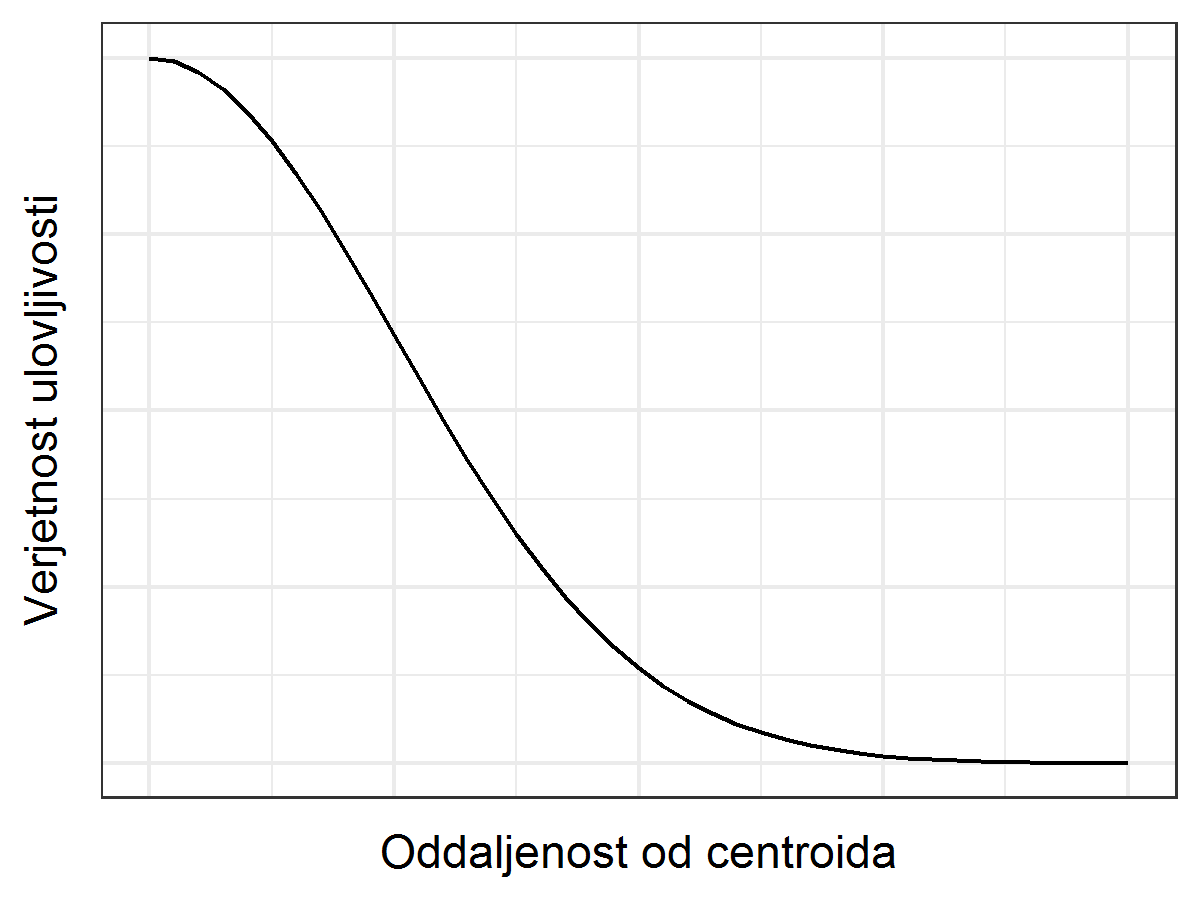
\includegraphics[width=0.5\linewidth]{../r_koda_slike/figures/half_normal.png}
  % \caption{A subfigure}
  \label{sli:sub2.1}
\end{subfigure}%
\begin{subfigure}{0.5\textwidth}
  \centering
  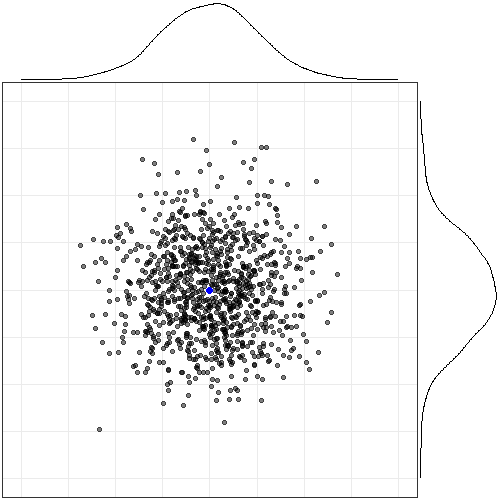
\includegraphics[width=0.5\linewidth]{../r_koda_slike/figures/homerange_usage.png}
  % \caption{A subfigure}
  \label{sli:sub2.2}
\end{subfigure}
\caption[Funkcija simuliranja vzorčnih točk]{Levo je ponazorjena verjetnost pojavljanja osebka oz. verjetnost, da ga zaznamo, v odvisnosti od oddaljenosti od centroida domačega okoliša. Prikaz desno ponazarja "ulov" osebka (sive pike) v prostoru, krivulje na desni in zgornji stranici pa sta robni gostoti.}
\label{sli:slika2}
\end{figure}

Osebkom, ki imajo pretežni delež domačega okoliša znotraj vzorčenega območja, lahko pripišemo delež njihovega domačega okoliša znotraj območja vzorčenja 1. V kolikor pa se centroid osebka nahaja v bližini roba območja vzorčenja, lahko pričakujemo, da bo del časa osebek preživel zunaj območja. V tem času med vzorčenjem ne bo zaznaven (ulovljiv), zato bo delež njegovega domačega okoliša znotraj območja vzorčenja manjši od 1. Podobno velja za krivulje, ki nimajo parametrične oblike (neparametrične krivulje).

Osebke med premikanjem lovimo in beležimo lokacijo in čas, ko smo jih zaznali. Točke na sliki \ref{sli:slika2} desno predstavljajo take ulove. Predpostavljamo, da te točke predstavljajo reprezentativno gibanje osebkov. Histogram razdalj med pari točk predstavlja razdalje, ki jih osebek lahko prehodi. To porazdelitev uporabimo pri izračunu deleža, ki pripada znotraj območja vzorčenja. Delež porazdelitve znotraj območja vzorčenja uporabimo v modelu kot individualno spremenljivko.

\subsubsection{Simulacije kot orodje za raziskovanje}
V matematičnih modelih opišemo pojav s funkcijami, ki so lahko preproste ali kompleksne. S kompleksnostjo pojava pa narašča tudi kompleksnost funkcij. Drug pristop je opis pojava s stohastičnimi procesi - simulacijami. Pojav razdelimo na manjše podenote in vsako enoto simuliramo kot samostojni proces. Razpon vrednosti, ki jih zavzemajo parametri podenote določi raziskovalec, najpogosteje na podlagi teoretskih osnov in poznavanje pojava. Podenota ni samostojna ampak je odvisna od drugih podenot in parametrov, ki jih določi raziskovalec. Primer take podenote je molekula vode, ki se obnaša na svoj način v razmerju do sosednjih molekul. Ko na sistem pogledamo od daleč lahko vidimo kako se le-ta obnaša glede na različne vhodne parametre. Na ta način simulirajo npr. ladijske elise, letalska krila ipd. V ekologiji lahko na tak način simuliramo gibanje in obnašanje živali ter preučujemo interakcijo med osebki oz. višjimi enotami in okoljem \citep{bolker_ecological_2008}.

\subsection{Cilji disertacije}
Cilj disertacije je izboljšati računanje gostote populacij, kjer med vzorčenjem prihaja do kršitve predpostavke o zaprtosti populacij.

Na podlagi razdalj med vzorčenimi lokacijami osebkov v območju vzorčenja bomo ocenili delež, ki ga osebek prebije znotraj območja vzorčenja. To informacijo bomo vključili v model za zaprte populacije kot individualno spremenljivko.

Ker bomo v modelu, ki upošteva individualno spremenljivko, v modeliranje vključili več informacij pričakujemo, da bo boljši od tistega, kjer te spremenljivke ne bomo uporabili. Za boljši model bomo smatrali tistega, ki bo imel nižji kriterij AICc.

Z vključitvijo informacije o morebitnem prehajanju roba vzorčenega območja v model, bomo izboljšali oceno ulovljivosti, saj bomo v model vključili eno od pomembnih komponent, ki vplivajo na spremenjeno zaznavnost in posledično ulovljivost osebkov. Pričakujemo, da bo model, ki vključuje individualno spremenljivko, uspešno kompenziral za spremenjeno ulovljivost zaradi prehoda čez rob območja vzorčenja.

Izboljšana ocena gostote bo na račun boljšega poznavanja velikosti dejanskega prispevka območja osebkov v območje vzorčenja, saj bomo iz gibanja osebkov lahko razbrali kako so razporejeni v prostoru.

Manjše kršitve predpostavke zaprtosti populacije ne bi smele bistveno vplivati na pristranskost ocene gostote. Pričakujemo, da bo razlika med ocenjeno in dejansko gostoto odvisna od razmerja med površino domačega okoliša in površino vzorčenega območja.
